\documentclass[11pt, letterpaper]{amsart}

\usepackage[latin1]{inputenc}
\usepackage[USenglish,british,american,australian,english]{babel}
\usepackage{amsmath,amssymb,amsfonts,amsthm}
\usepackage{graphicx}
\usepackage[T1]{fontenc}

\usepackage{braket}
\usepackage{mathrsfs}
\usepackage{subfigure}
\usepackage{listings}
\usepackage{lettrine}
\usepackage{epigraph}
\usepackage{wrapfig}
\usepackage{bm}
\usepackage[font={scriptsize,sl},format=hang,labelfont={sf,bf}]{caption}
\usepackage[final]{hyperref}
\usepackage{cite}
\usepackage[margin=1in,letterpaper]{geometry}
\usepackage{url}

\newcommand\norm[1]{\left\lVert#1\right\rVert}

\hyphenpenalty=20000
\tolerance=10000
\hbadness=10000

\title{Simulation of fluid flow in a Tesla valve}
\author{Hatef Khadivinassab, Daniele Rizzi}
\date{July 2, 2020}

\begin{document}
\maketitle
%---------------CHANGES---------------%
%07-17 Modified Title, Introduction, Tesla valve

%-----------------------------------------------------------------------------------------------------------------
\section{Introduction}
The use of microvalve to move small quantities of fluid has great importance in medicine, such as for example in drug delivery and in cardiology, in biotechnology, such as for handling biomolecules, and in chemistry\cite{microvalve}\cite{actuator_valves}. In these applications,the ability to control and move milli and micro liters of fluid has great importance, together with the ability to predict the behavior of the flow inside the valves.
\newline
Microvalves may be divided in two major categories, active and passive. Active valves use moving parts such as mechanical moving membranes that are coupled by magnetic, electric, piezoelectric or thermal actuation methods\cite{microvalve}.
Passive valves are characterized by not having any moving part and their operational state (open or closed) is directly determined by the fluid.

\begin{figure}[!h]
\centering%
\subfigure[\label{fig:activevalve}]%
{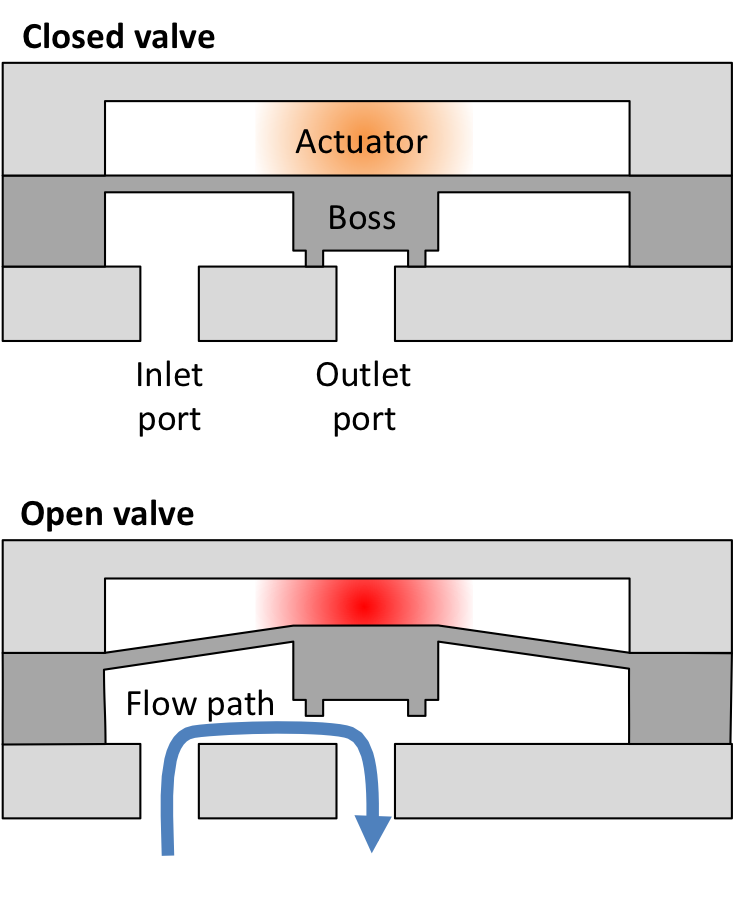
\includegraphics[angle=0,width=0.3\linewidth]{active_valve.png}}\qquad\qquad
\subfigure[\label{fig:passivevalve}]%
{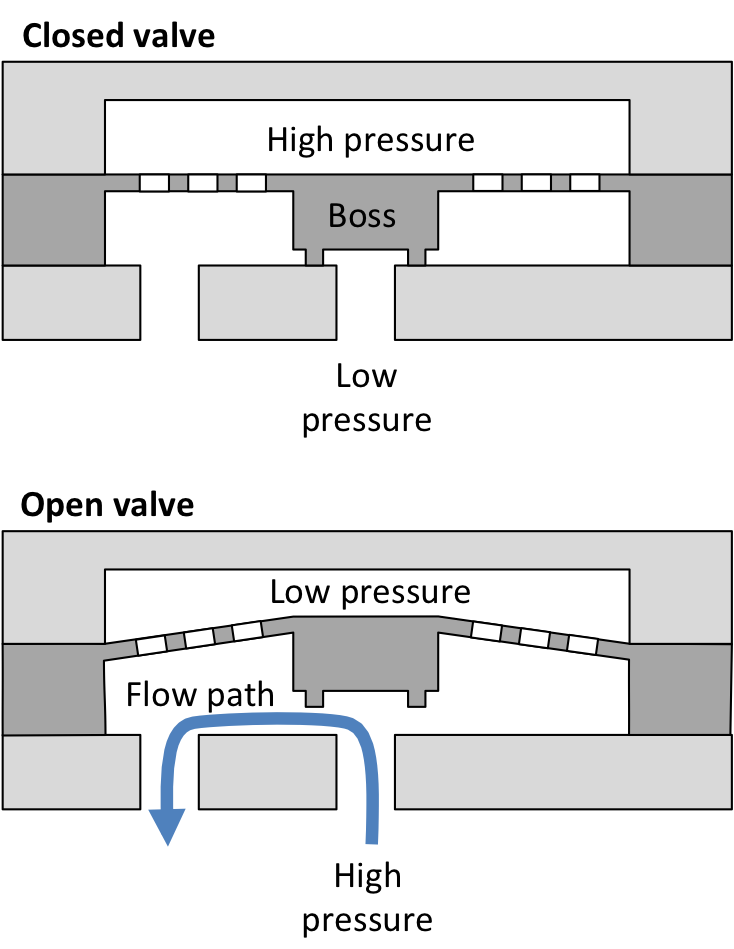
\includegraphics[angle=0,width=0.3\linewidth]{passive_valve.png}}
\caption{Functional scheme of active (a) and passive (b) valves. Source \url{https://en.wikipedia.org/wiki/Microvalve}. \label{fig:valves}}
\end{figure}

Many microvalves have advantages such as low cost, ease of fabrication and scalability, characteristics that contribute to their increasing usage in industry and medicine.
Despite all these advantages, their operation is characterized by the equations of moving fluids in the form of the Navier-Stokes equation, whose solution is still an open problem in the field of mathematics. To predict the behavior of a moving fluid, a Computational Fluid Dynamics Simulation must be performed, whose aim is to solve numerically the equation of fluids to obtain informations about the flow such as velocity and pressure of the fluid.
\newline
In this paper we will analyse and discuss the diodicity of a Tesla valve with a CFD simulation using the open source computing platform FEniCS.

%-----------------------------------------------------------------------------------------------------------------
\section{Tesla valve}
One of the first design of micro valves is due to Nikola Tesla who patented a passive valve that allows flow preferentially in one direction, while it prevents flow in the other direction.
The basic design of this valve consists of channel that is splitted in a Y junction that re-enters in a T channel.
This valve has many advantages since it is easy to design, easy to fabricate and it can be scaled with ease.

\begin{figure}[!h]
\begin{centering}
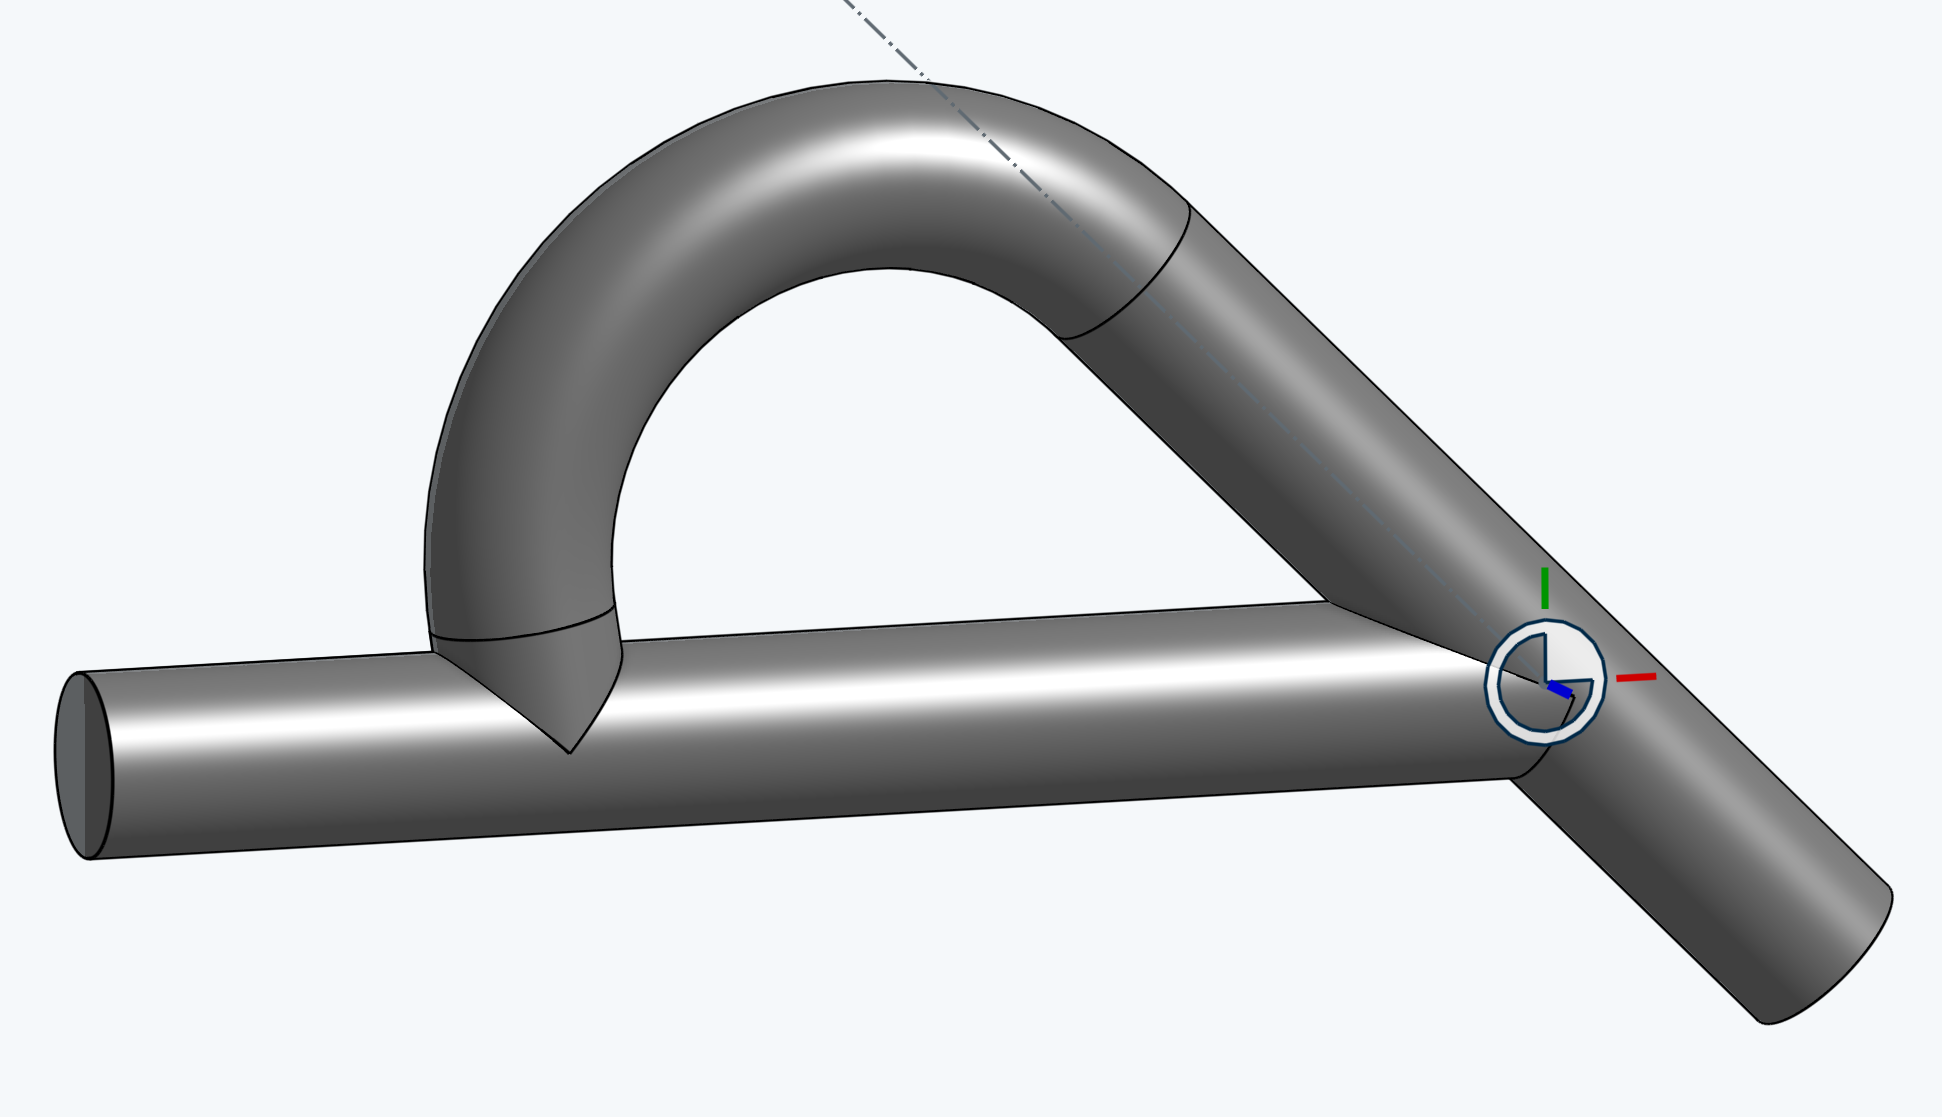
\includegraphics[angle=0,width=0.5\linewidth]{tesla-valve.png}
\par\end{centering}
\caption{Tesla valve design used for this simulation}
\label{fig:tesla-valve}
\end{figure}

\begin{figure}[!h]
\begin{centering}
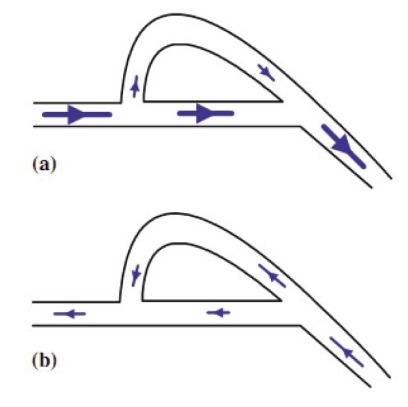
\includegraphics[angle=0,width=0.5\linewidth]{tesla_flow.png}
\par\end{centering}
\caption{Flow in a tesla valve in forward (a) and reverse (b) direction\cite{tesla_valve}}
\label{fig:tesla-flow}
\end{figure}

Such a valve, named after its inventor, is structured to have a higher pressure drop for the flow in one direction (reverse) than the other (forward). This difference in flow resistance causes a net directional flow rate in the forward direction in oscillating flows. The efficiency is often expressed in terms of the diodicity $D_i$, defined as the ratio of pressure drops for identical flow rates

\begin{equation}
D_i = \left({\frac {\Delta p_{r}}{\Delta p_{f}}}\right)_{Q}
\end{equation}

where $\Delta p_{r}$ is the reverse flow pressure drop and $\Delta p_{f}$ the forward flow pressure drop for flow rate.
Since the diodicity of such valve depends on the pressure drop between direct flow versus the reverse flow, higher diodicity values may be obtained by changing geometrical parameters of this type of valve, such as

\begin{itemize}
\item angle between channel and T junction
\item angle between channel and Y junction
\item number of branches of the valve
\end{itemize}

\bigskip
%-----------------------------------------------------------------------------------------------------------------
\section{Problem definition}
The flow equations are the Navier Stokes equations for incompressible flow, which in the weak form can be stated as

\begin{eqnarray}
\dot{u} + \nabla u \cdot u - \nu \Delta u + \nabla p & = & f\\
\nabla \cdot u & = & 0
\end{eqnarray}

where $u$ is the unknown velocity, $p$ is the pressure field, $\nu$ is the given kinematic viscosity and $f$ a given source.

paired with Dirichlet and Neumann boundary conditions that we will describe later.

The Navier Stokes equations can be rewritten in the finite element weak form as

\begin{equation}
F = \left(\frac{u - u_0}{dt}, v \right) + \left(\nabla u_m \cdot u_m, v \right) + \nu \left(\nabla u_m, \nabla v \right) + \left(\nabla p, v \right) + \left(\nabla \cdot u_m, q \right) - \left(f,v \right)
\end{equation}

where $u_m = \theta u + (1-\theta) u_0$ with $\theta = 0.5$ in the Crank-Nicholson scheme.

\subsection{Stabilization methods}

It is well known that the numerical solution of Navier-Stokes equations using Finite Element Methods suffers from two sources of numerical instabilities\cite{tezduyar}\cite{tezduyar2}

\begin{itemize}
	\item using wrong combination of velocity and pressure finite element spaces (that do not satisfy the inf-sup condition) generate numerical oscillations in the pressure field (spurious pressure)
	\item when the problem is convection-dominated ($Re >> 1$), numerical oscllations in the velocity field occurs (called spurious velocity).
\end{itemize}

\bigskip

These sources of instabilities may be controlled in two ways

\begin{itemize}
	\item using appropriate combination of velocity and pressure finite element spaces
	\item adding stabilization terms to the weak formulation of the problem
\end{itemize}

The first item can be addressed by using a $P_k$-$P_k+1$ combination of spaces for the unknown fields velocity and pressure.
Such mixed formulation is expressed in FEniCS with the following lines of code, in which the Vector Element space $Q_e = P_1$ for the pressure and the space $V_e = P_2$ for the velocity and mixed in the space $W = V_e Q_e = P_k P_{k+1} = P_1 P_2$.

\bigskip
\begin{verbatim}
    Ve = VectorElement("CG", mesh.ufl_cell(), 2)
    Qe = FiniteElement("CG", mesh.ufl_cell(), 1)
    W = FunctionSpace(mesh, Ve * Qe)

    # Define test functions
    w = Function(W)
    u, p = split(w)
    (v, q) = TestFunctions(W)
    w0 = Function(W)
    u0, _ = split(w0)
\end{verbatim}
\bigskip

The second way to reduce numerical instabilities is to add to the weak formulation a stabilization term as expressed in \cite{tezduyar}, \cite{tezduyar2} and \cite{jansson_aircraft}. In our formulation the stabilization term is the following 

\begin{equation}
F_{stabilization} = \tau \left[\left(\nabla p + \nabla u_m \cdot u_m - f, \nabla q + \nabla v \cdot u_ m \right) + \left(\nabla \cdot u_m, \nabla \cdot v\right)\right]
\end{equation}

where $\tau$ is the stabilization parameter defined as

\begin{equation}
\tau = \left[\left(\frac{2}{dt} \right)^2 + \left(\frac{2 \norm{u}}{h} \right)^2  \left(\frac{4 \nu}{h^2} \right)^2   \right]^{(-0.5)}
\end{equation}

in which $h$ is defined as the mean mesh cell diameter.

%-----------------------------------------------------------------------------------------------------------------
\section{Geometry}
The Tesla valve has been designed following the geometry provided in \cite{gamboa_valve}, with the following dimensions
\textbf{ADD DIMENSIONS}

\begin{figure}[!h]
\begin{centering}
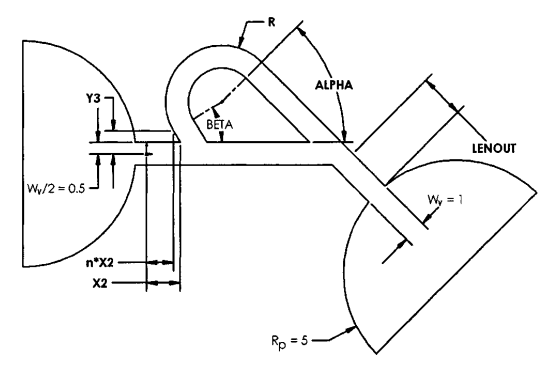
\includegraphics[angle=0,width=8cm]{tesla_geometry.png}
\par\end{centering}
\caption{Design of tesla valve provided in  \cite{gamboa_valve}}
\label{fig:tesla-geometry}
\end{figure}

%-----------------------------------------------------------------------------------------------------------------
\section{Software}
The CAD geometry has been designed using OnShape whose 3D step file has been imported into GmSH to define the mesh and surface boundaries.
The calculations are performed using FEniCS open source computing platform and Paraview for the visualization of the results.

%-----------------------------------------------------------------------------------------------------------------
\section{Numerical simulation}
The simulation is performed by evaluating the flow of a fluid with viscosity $\nu = $.
The inlet velocity is assumed to have velocity only along the x-axis with a parabolic profile with the following shape

\begin{equation}
v_{in} = \frac{4U y\left( R-y \right) z\left(R-z \right)}{R^4}
\end{equation}

where $R$ is the radius of the conduct and $U$ is the maximum value of the velocity profile.
Velocity components along y and z are supposed to have zero value.
Dirichlet no-slip condition is applied on the walls of the valve.


%-----------------------------------------------------------------------------------------------------------------
\section{Results and discussion}





%-----------------------------------------------------------------------------------------------------------------
\begin{thebibliography}{99}
\bibitem{microvalve}
	Kwang, Chong,emph{A review of microvalves}, J. Micromech. Microeng. $16$ $(2006)$
\bibitem{actuator_valves}
	Jin-Yuan Qian, Cong-Wei Hou, Xiao-Juan Li and Zhi-Jiang Jin, \emph{Actuation Mechanism of Microvalves: A Review}, Micromachines $2020$, $11$, $172$\bibitem{tesla_valve}
	A. Y. Nobakht, M. Shahsavan, A. Paykani,
	\emph{Numerical Study of Diodicity Mechanism in Different Tesla-Type Microvalves}, Journal of Applied Research and Technology, Vol.$11$, December $2013$
\bibitem{tezduyar}
	T.E. Tezduyar,
	\emph{Stabilized finite element formulations for incompressible flow computations}, Advances in Applied Mechanics, 28 (1992) 1-44
\bibitem{tezduyar2}
	T.E. Tezduyar, S. Mittal, S.E. Ray and R. Shih,
	\emph{Incompressible flow computations with stabilized bilinear and linear equal-order-interpolation velocity-pressure elements}, Computer Methods in Applied Mechanics and Engineering, 95 (1992) 221-242
\bibitem{jansson_aircraft}
    J. Jansson, E. Krishnasamy, M. Leoni, N. Jansson and J. Hoffman,
    \emph{Time-resolved Adaptive Direct FEM Simulation of High-lift Aircraft Configurations}
\bibitem{logg_fenics}
	A. Logg, H. P. Langtangen,
	\emph{Solving PDEs in Python}, Springer $2017$
\bibitem{fenics_book}
	A. Logg, K. A. Mardal, G. N. Wells,
	\emph{Automated Solution of Differential Equations by the Finite Element Method}, Springer $2017$
\bibitem{gamboa_valve}
	A. Gamboa, C. Morris, F. Foster,
	\emph{Improvements in Fixed-Valve Micropump Performance Through Shape Optimization of Valves}, Journal of Fluids Engineering, March $2005$, Vol. $127$
\end{thebibliography}

\end{document}